\documentclass[12pt,a4paper]{article}

%\usepackage[left=1.5cm,right=1.5cm,top=1cm,bottom=2cm]{geometry}
\usepackage[in, plain]{fullpage}
\usepackage{array}
\usepackage{../../../pas-math}
\usepackage{../../../moncours}


%\usepackage{pas-cours}
%-------------------------------------------------------------------------------
%          -Packages nécessaires pour écrire en Français et en UTF8-
%-------------------------------------------------------------------------------
\usepackage[utf8]{inputenc}
\usepackage[frenchb]{babel}
\usepackage[T1]{fontenc}
\usepackage{lmodern}
\usepackage{textcomp}



%-------------------------------------------------------------------------------

%-------------------------------------------------------------------------------
%                          -Outils de mise en forme-
%-------------------------------------------------------------------------------
\usepackage{hyperref}
\hypersetup{pdfstartview=XYZ}
%\usepackage{enumerate}
\usepackage{graphicx}
\usepackage{multicol}
\usepackage{tabularx}
\usepackage{multirow}


\usepackage{anysize} %%pour pouvoir mettre les marges qu'on veut
%\marginsize{2.5cm}{2.5cm}{2.5cm}{2.5cm}

\usepackage{indentfirst} %%pour que les premier paragraphes soient aussi indentés
\usepackage{verbatim}
\usepackage{enumitem}
\usepackage[usenames,dvipsnames,svgnames,table]{xcolor}

\usepackage{variations}

%-------------------------------------------------------------------------------


%-------------------------------------------------------------------------------
%                  -Nécessaires pour écrire des mathématiques-
%-------------------------------------------------------------------------------
\usepackage{amsfonts}
\usepackage{amssymb}
\usepackage{amsmath}
\usepackage{amsthm}
\usepackage{tikz}
\usepackage{xlop}
%-------------------------------------------------------------------------------



%-------------------------------------------------------------------------------


%-------------------------------------------------------------------------------
%                    - Mise en forme avancée
%-------------------------------------------------------------------------------

\usepackage{ifthen}
\usepackage{ifmtarg}


\newcommand{\ifTrue}[2]{\ifthenelse{\equal{#1}{true}}{#2}{$\qquad \qquad$}}

%-------------------------------------------------------------------------------

%-------------------------------------------------------------------------------
%                     -Mise en forme d'exercices-
%-------------------------------------------------------------------------------
%\newtheoremstyle{exostyle}
%{\topsep}% espace avant
%{\topsep}% espace apres
%{}% Police utilisee par le style de thm
%{}% Indentation (vide = aucune, \parindent = indentation paragraphe)
%{\bfseries}% Police du titre de thm
%{.}% Signe de ponctuation apres le titre du thm
%{ }% Espace apres le titre du thm (\newline = linebreak)
%{\thmname{#1}\thmnumber{ #2}\thmnote{. \normalfont{\textit{#3}}}}% composants du titre du thm : \thmname = nom du thm, \thmnumber = numéro du thm, \thmnote = sous-titre du thm

%\theoremstyle{exostyle}
%\newtheorem{exercice}{Exercice}
%
%\newenvironment{questions}{
%\begin{enumerate}[\hspace{12pt}\bfseries\itshape a.]}{\end{enumerate}
%} %mettre un 1 à la place du a si on veut des numéros au lieu de lettres pour les questions 
%-------------------------------------------------------------------------------

%-------------------------------------------------------------------------------
%                    - Mise en forme de tableaux -
%-------------------------------------------------------------------------------

\renewcommand{\arraystretch}{1.7}

\setlength{\tabcolsep}{1.2cm}

%-------------------------------------------------------------------------------



%-------------------------------------------------------------------------------
%                    - Racourcis d'écriture -
%-------------------------------------------------------------------------------

% Angles orientés (couples de vecteurs)
\newcommand{\aopp}[2]{(\vec{#1}, \vec{#2})} %Les deuc vecteurs sont positifs
\newcommand{\aopn}[2]{(\vec{#1}, -\vec{#2})} %Le second vecteur est négatif
\newcommand{\aonp}[2]{(-\vec{#1}, \vec{#2})} %Le premier vecteur est négatif
\newcommand{\aonn}[2]{(-\vec{#1}, -\vec{#2})} %Les deux vecteurs sont négatifs

%Ensembles mathématiques
\newcommand{\naturels}{\mathbb{N}} %Nombres naturels
\newcommand{\relatifs}{\mathbb{Z}} %Nombres relatifs
\newcommand{\rationnels}{\mathbb{Q}} %Nombres rationnels
\newcommand{\reels}{\mathbb{R}} %Nombres réels
\newcommand{\complexes}{\mathbb{C}} %Nombres complexes


%Intégration des parenthèses aux cosinus
\newcommand{\cosP}[1]{\cos\left(#1\right)}
\newcommand{\sinP}[1]{\sin\left(#1\right)}


%Probas stats
\newcommand{\stat}{statistique}
\newcommand{\stats}{statistiques}
%-------------------------------------------------------------------------------

%-------------------------------------------------------------------------------
%                    - Mise en page -
%-------------------------------------------------------------------------------

\newcommand{\twoCol}[1]{\begin{multicols}{2}#1\end{multicols}}


\setenumerate[1]{font=\bfseries,label=\textit{\alph*})}
\setenumerate[2]{font=\bfseries,label=\arabic*)}


%-------------------------------------------------------------------------------
%                    - Elements cours -
%-------------------------------------------------------------------------------





%\makeatletter
%\renewcommand*{\@seccntformat}[1]{\csname the#1\endcsname\hspace{0.1cm}}
%\makeatother


%\author{Olivier FINOT}
\date{}
\title{}

%\newcommand{\disp}{false}

%
%\rfoot{Page \thepage}
\begin{document}
	%\maketitle
	\chap[num=4, color=red]{Notion de fonction}{Olivier FINOT, \today }


\section{Définition et vocabulaire}


\begin{mydefs}
	
	
	
	\begin{itemize}
		\item Une fonction est un \kw{procédé} qui permet de faire correspondre à un nombre de départ $x$, un autre nombre qui en dépend. Le procédé peut être \kw{une formule}, c'est à dire une suite de calculs qui dépend de $x$.
		
		\item Toute fonction est définie sur \kw{intervalle} (entre une valeur minimale et une valeur maximale).
		
		\item Elle a un nom, souvent \kw{$f$}.
		
		\item Le nombre de départ, est en général appelé $x$. Le nombre qui lui est associé est alors noté \kw{$f(x)$}.
		
		\item Le nombre $f(x)$ est appelé \kw{image de $x$} par la fonction $f$.
		
		\item \kw{x} est appelé \kw{antécédent de $f(x)$} par la fonction $f$
		
		\item $f$ est croissante si $ \forall a, b \in I.$ $ a \leq b \Leftrightarrow f(a) \leq f(b) $ 
	\end{itemize}
	
	
	

\end{mydefs}

	\begin{myex}
		La fonction $f$, qui a toute valeur d'un nombre $x$, fait correspondre $x^2-1$ est notée :
		\kw{\begin{align*}
			f(x) = x^2-1
		\end{align*}}	
	\begin{itemize}
		\item L'image de $2$ par $f$ est : $f(2) = 2^2-1=3$
		\item L'image de $-2$ par $f$ est : $f(-2) = (-2)^2-1=3$
		\item[$\rightarrow$] $-2$ et $2$ sont des antécédents de $3$ par $f$.
		
	\end{itemize}
	\end{myex}

\section{Représentation graphique d'une fonction}

\subsection{Courbe représentative}

\begin{mydef}
	La courbe représentative de la fonction $f$ défine sur l'intervalle $[a;b]$ est l'ensemble des points de coordonnées $(x;f(x))$, où $x$ varie entre $a$ et $b$.
\end{mydef}

\begin{myex}
	\begin{multicols}{2}
		La courbe ci-contre est la représentation graphique de la fonction $f(x)=x^2-1$ entre $-2$ et $2$ (sur l'intervalle $[-2;2]$).
		
		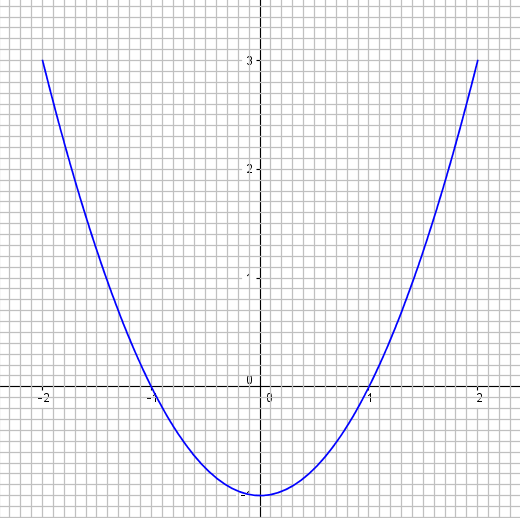
\includegraphics[scale=0.4]{img/ex1}
	\end{multicols}
	
\end{myex}
	
\subsection{Lecture graphique}

\begin{myprops}
	\begin{itemize}
		\item L'\kw{image} d'un nombre se lit sur l'axe des \kw{ordonnées}.
		\item L'\kw{antécédent} d'un nombre se lit sur l'axe des \kw{abscisses}.
	\end{itemize}
\end{myprops}


\begin{mymeth}
	
	\begin{multicols}{2}
		
	
		Pour lire l'image d'un nombre $a$ :
		\begin{enumerate}
			\item Repérer $b$ sur l'axe des abscisses;
			\item Rejoindre la courbe verticalement;
			\item Repérer la valeur correspondante sur l'axe des ordonnées, $f(a)$.
		\end{enumerate}
		
		
		Pour lire l'antécédent d'un nombre $b$ :
		\begin{enumerate}
			\item Repérer $b$ sur l'axe des ordonnées;
			\item Rejoindre la courbe horizontalement;
			\item Repérer la valeur correspondante sur l'axe des abscisses.
		\end{enumerate}
		
		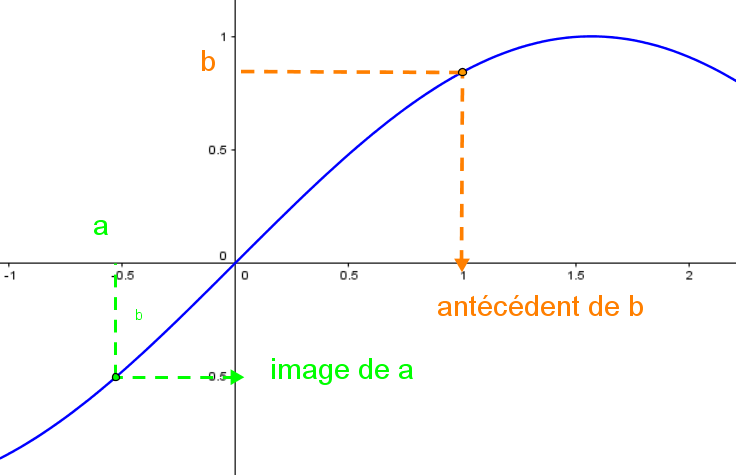
\includegraphics[scale=0.5]{img/graph2}
	\end{multicols}
\end{mymeth}

\end{document}	